\begin{figure*}
    \centering
    \resizebox{1.000\textwidth}{!}{
        \begin{tikzpicture}[
                legendLabel/.style={right, inner sep=1, text=white, thin, draw=black, rounded corners=2, xshift=0.1cm, minimum height=0.25cm}
        ]
        \definecolor{darkGray}{RGB}{71, 79, 82}   

        \definecolor{darkRed}{RGB}{150, 0, 25}
        \definecolor{darkBrown}{RGB}{150, 75, 0}
        \definecolor{darkGreen}{RGB}{25, 125, 0}
        \definecolor{darkBlue}{RGB}{0, 25, 150}      
        \definecolor{darkPurple}{RGB}{150, 0, 150}   

        \definecolor{darkCyan}{RGB}{0, 125, 125}

        \node[draw, fill=darkGray, text=white, minimum width=10cm, minimum height=0.5cm, inner sep=0, anchor=west] at (-1.75cm, 5.25cm) {\textbf{GEMM}};
        \node[draw, minimum width=10cm, minimum height=6cm, inner sep=0, anchor=north west] at (-1.75cm, 5cm) {};
        \node[draw, fill=darkGray, text=white, minimum width=10cm, minimum height=0.5cm, inner sep=0, anchor=west] at (-1.75cm+10cm, 5.25cm) {\textbf{ATAX}};
        \node[draw, minimum width=10cm, minimum height=6cm, inner sep=0, anchor=north west] at (-1.75cm+10cm, 5cm) {};
        \node[draw, fill=darkGray, text=white, minimum width=10cm, minimum height=0.5cm, inner sep=0, anchor=west] at (-1.75cm+20cm, 5.25cm) {\textbf{GESUMMV}};
        \node[draw, minimum width=10cm, minimum height=6cm, inner sep=0, anchor=north west] at (-1.75cm+20cm, 5cm) {};
        \node[draw, fill=darkGray, text=white, minimum width=10cm, minimum height=0.5cm, inner sep=0, anchor=west] at (-1.75cm, 5.25cm-6.5cm) {\textbf{MVT}};
        \node[draw, minimum width=10cm, minimum height=6cm, inner sep=0, anchor=north west] at (-1.75cm, 5cm-6.5cm) {};
        \node[draw, fill=darkGray, text=white, minimum width=10cm, minimum height=0.5cm, inner sep=0, anchor=west] at (-1.75cm+10cm, 5.25cm-6.5cm) {\textbf{TRISOLV}};
        \node[draw, minimum width=10cm, minimum height=6cm, inner sep=0, anchor=north west] at (-1.75cm+10cm, 5cm-6.5cm) {};
        \node[draw, fill=darkGray, text=white, minimum width=10cm, minimum height=0.5cm, inner sep=0, anchor=west] at (-1.75cm+20cm, 5.25cm-6.5cm) {\textbf{TRSM}};
        \node[draw, minimum width=10cm, minimum height=6cm, inner sep=0, anchor=north west] at (-1.75cm+20cm, 5cm-6.5cm) {};

        \begin{axis}[
            width=8cm,
            height=6.0cm,
            xlabel={Input Matrix Size},
            ylabel={Latency [cycles]},
            xmin=0,
            xmax=23,
            xtick={4,8,20},
            xticklabels={4$\times$4,8$\times$8,20$\times$20,32$\times$32},
            grid=major,
            %ymode=log,
            clip = false,
            clip mode=individual
            % If you want to force axis to exactly match your data points:
            % xtick distance=4,
            % scaled x ticks=false
        ]

            % TCPA-Period
            \addplot[
                smooth,  % Makes the line smooth
                darkGray,
                thick,
                mark=*,  % Filled circle markers
                dashed,
                mark options={solid}
            ] coordinates {
                (4, 80)
                (8,40)
                (20,525)
            }coordinate[pos=1.0] (tcpaPeriod);
            \node [legendLabel, fill=darkGray] (labelNode) at ([xshift=0.1cm, yshift=-0.30cm]tcpaPeriod)  {TURTLE (first)};
            \draw[densely dotted, darkGray] (tcpaPeriod) -- (labelNode.west);

            % TCPA
            \addplot[
                smooth,  % Makes the line smooth
                darkGray,
                thick,
                mark=*,  % Filled circle markers
                dashed,
                mark options={solid}
            ] coordinates {
                (4, 81)
                (8,108)
                (20,639)
            }coordinate[pos=1.0] (tcpa);
            \node [legendLabel, fill=darkGray] (labelNode) at ([xshift=0.1cm, yshift=0.1cm]tcpa)  {TURTLE (last)};
            \draw[densely dotted, darkGray] (tcpa) -- (labelNode.west);

            % Morpher
            \addplot[
                %smooth,  % Makes the line smooth
                darkGray,
                thick,
                mark=*,  % Filled circle markers
                dashed,
                mark options={solid}
            ] coordinates {
                (4,141)
                (8,1037)
                (20,16013)
                %(32,65549)
            }coordinate[pos=1.0] (morpher);
            \node [legendLabel, fill=darkGray] (labelNode) at ([xshift=0.1cm]morpher)  {Morpher};
            \draw[densely dotted, darkGray] (morpher) -- (labelNode.west);

            % CGRA-Flow
            \addplot[
                %smooth,  % Makes the line smooth
                darkGray,
                thick,
                mark=*,  % Filled circle markers
                dashed,
                mark options={solid}
            ] coordinates {
                (4,127)
                (8,799)
                (20,12031)
                %(32,49183)
            }coordinate[pos=1.0] (cgraFlow);
            \node [legendLabel, fill=darkGray] (labelNode) at ([xshift=0.1cm]cgraFlow)  {CGRA-Flow};
            \draw[densely dotted, darkGray] (cgraFlow) -- (labelNode.west);

            \draw[{Latex[length=0.25cm]}-, line cap=round, line width=0.075cm, red] let \p1 = (tcpa), \p2 = (cgraFlow) in ([xshift=0.0cm]cgraFlow) -- node[right] {\pgfmathparse{int(round(1 / (1 - (1 - \y1 / \y2))))} \scriptsize \textbf{19$\times$}} ([xshift=0.0cm]tcpa);

        \end{axis}

        \begin{axis}[
            xshift=10cm,
            width=8cm,
            height=6.0cm,
            xlabel={Input Matrix Size},
            ylabel={Latency [cycles]},
            xmin=0,
            xmax=35,
            xtick={4,8,20,32},
            xticklabels={4$\times$4,8$\times$8,20$\times$20,32$\times$32},
            grid=major,
            %ymode=log,
            clip = false,
            clip mode=individual
            % If you want to force axis to exactly match your data points:
            % xtick distance=4,
            % scaled x ticks=false
        ]

            % TCPA-Period
            \addplot[
                smooth,  % Makes the line smooth
                darkGray,
                thick,
                mark=*,  % Filled circle markers
                dashed,
                mark options={solid}
            ] coordinates {
                (4,18)
                (8,36)
                (20,180)
                (32,432)
            }coordinate[pos=1.0] (tcpaPeriod);
            \node [legendLabel, fill=darkGray] (labelNode) at ([xshift=0.1cm, yshift=-0.1cm]tcpaPeriod)  {TURTLE (first)};
            \draw[densely dotted, darkGray] (tcpaPeriod) -- (labelNode.west);

            % TCPA
            \addplot[
                smooth,  % Makes the line smooth
                darkGray,
                thick,
                mark=*,  % Filled circle markers
                dashed,
                mark options={solid}
            ] coordinates {
                (4,107)
                (8,183)
                (20,689)
                (32,1641)
            }coordinate[pos=1.0] (tcpa);
            \node [legendLabel, fill=darkGray] (labelNode) at ([xshift=0.1cm]tcpa)  {TURTLE (last)};
            \draw[densely dotted, darkGray] (tcpa) -- (labelNode.west);

            % Morpher
            \addplot[
                smooth,  % Makes the line smooth
                darkGray,
                thick,
                mark=*,  % Filled circle markers
                dashed,
                mark options={solid}
            ] coordinates {
                (4,121)
                (8,457)
                (20,2809)
                (32,7177)
            }coordinate[pos=1.0] (morpher);
            \node [legendLabel, fill=darkGray] (labelNode) at ([xshift=0.1cm]morpher)  {Morpher};
            \draw[densely dotted, darkGray] (morpher) -- (labelNode.west);

            % CGRA-Flow
            \addplot[
                smooth,  % Makes the line smooth
                darkGray,
                thick,
                mark=*,  % Filled circle markers
                dashed,
                mark options={solid}
            ] coordinates {
                (4,215)
                (8,815)
                (20,5015)
                (32,12815)
            }coordinate[pos=1.0] (cgraFlow);
            \node [legendLabel, fill=darkGray] (labelNode) at ([xshift=0.1cm]cgraFlow)  {CGRA-Flow};
            \draw[densely dotted, darkGray] (cgraFlow) -- (labelNode.west);

            \draw[{Latex[length=0.25cm]}-, line cap=round, line width=0.075cm, red] let \p1 = (tcpa), \p2 = (morpher) in ([xshift=0.0cm]morpher) -- node[right] {\pgfmathparse{int(round(1 / (1 - (1 - \y1 / \y2))))} \scriptsize \textbf{4$\times$}} ([xshift=0.0cm]tcpa);

        \end{axis}

        \begin{axis}[
            xshift=20cm,
            width=8cm,
            height=6.0cm,
            xlabel={Input Matrix Size},
            ylabel={Latency [cycles]},
            xmin=0,
            xmax=35,
            xtick={4,8,20,32},
            xticklabels={4$\times$4,8$\times$8,20$\times$20,32$\times$32},
            grid=major,
            %ymode=log,
            clip = false,
            clip mode=individual
            % If you want to force axis to exactly match your data points:
            % xtick distance=4,
            % scaled x ticks=false
        ]

            % TCPA-Period
            \addplot[
                smooth,  % Makes the line smooth
                darkGray,
                thick,
                mark=*,  % Filled circle markers
                dashed,
                mark options={solid}
            ] coordinates {
                (4,12)
                (8,36)
                (20,180)
                (32,432)
            }coordinate[pos=1.0] (tcpaPeriod);
            \node [legendLabel, fill=darkGray] (labelNode) at ([xshift=0.1cm, yshift=-0.2cm]tcpaPeriod)  {TURTLE (first)};
            \draw[densely dotted, darkGray] (tcpaPeriod) -- (labelNode.west);

            % TCPA
            \addplot[
                smooth,  % Makes the line smooth
                darkGray,
                thick,
                mark=*,  % Filled circle markers
                dashed,
                mark options={solid}
            ] coordinates {
                (4,96)
                (8,134)
                (20,318)
                (32,624)
            }coordinate[pos=1.0] (tcpa);
            \node [legendLabel, fill=darkGray] (labelNode) at ([xshift=0.1cm]tcpa)  {TURTLE (last)};
            \draw[densely dotted, darkGray] (tcpa) -- (labelNode.west);

            % Morpher
            \addplot[
                smooth,  % Makes the line smooth
                darkGray,
                thick,
                mark=*,  % Filled circle markers
                dashed,
                mark options={solid}
            ] coordinates {
                (4,56)
                (8,164)
                (20,920)
                (32,2324)
            }coordinate[pos=1.0] (morpher);
            \node [legendLabel, fill=darkGray] (labelNode) at ([xshift=0.1cm]morpher)  {Morpher};
            \draw[densely dotted, darkGray] (morpher) -- (labelNode.west);

            % CGRA-Flow
            \addplot[
                smooth,  % Makes the line smooth
                darkGray,
                thick,
                mark=*,  % Filled circle markers
                dashed,
                mark options={solid}
            ] coordinates {
                (4,56)
                (8,140)
                (20,728)
                (32,1820)
            }coordinate[pos=1.0] (cgraFlow);
            \node [legendLabel, fill=darkGray] (labelNode) at ([xshift=0.1cm]cgraFlow)  {CGRA-Flow};
            \draw[densely dotted, darkGray] (cgraFlow) -- (labelNode.west);

            \draw[{Latex[length=0.25cm]}-, line cap=round, line width=0.075cm, red] let \p1 = (tcpa), \p2 = (cgraFlow) in ([xshift=0.0cm]cgraFlow) -- node[right] {\pgfmathparse{int(round(1 / (1 - (1 - \y1 / \y2))))} \scriptsize \textbf{3$\times$}} ([xshift=0.0cm]tcpa);

        \end{axis}
        \begin{axis}[
            xshift=0cm,
            yshift=-6.5cm,
            width=8cm,
            height=6.0cm,
            xlabel={Input Matrix Size},
            ylabel={Latency [cycles]},
            xmin=0,
            xmax=35,
            xtick={4,8,20,32},
            xticklabels={4$\times$4,8$\times$8,20$\times$20,32$\times$32},
            grid=major,
            %ymode=log,
            clip = false,
            clip mode=individual
            % If you want to force axis to exactly match your data points:
            % xtick distance=4,
            % scaled x ticks=false
        ]

            % TCPA-Period
            \addplot[
                smooth,  % Makes the line smooth
                darkGray,
                thick,
                mark=*,  % Filled circle markers
                dashed,
                mark options={solid}
            ] coordinates {
                (4,9)
                (8,18)
                (20,90)
                (32,216)
            }coordinate[pos=1.0] (tcpaPeriod);
            \node [legendLabel, fill=darkGray] (labelNode) at ([xshift=0.1cm]tcpaPeriod)  {TURTLE (first)};
            \draw[densely dotted, darkGray] (tcpaPeriod) -- (labelNode.west);

            % TCPA
            \addplot[
                smooth,  % Makes the line smooth
                darkGray,
                thick,
                mark=*,  % Filled circle markers
                dashed,
                mark options={solid}
            ] coordinates {
                (4,81)
                (8,117)
                (20,372)
                (32,849)
            }coordinate[pos=1.0] (tcpa);
            \node [legendLabel, fill=darkGray] (labelNode) at ([xshift=0.1cm]tcpa)  {TURTLE (last)};
            \draw[densely dotted, darkGray] (tcpa) -- (labelNode.west);

            % Morpher
            \addplot[
                smooth,  % Makes the line smooth
                darkGray,
                thick,
                mark=*,  % Filled circle markers
                dashed,
                mark options={solid}
            ] coordinates {
                (4,49)
                (8,145)
                (20,817)
                (32,2065)
            }coordinate[pos=1.0] (morpher);
            \node [legendLabel, fill=darkGray] (labelNode) at ([xshift=0.1cm]morpher)  {Morpher};
            \draw[densely dotted, darkGray] (morpher) -- (labelNode.west);

            % CGRA-Flow
            \addplot[
                smooth,  % Makes the line smooth
                darkGray,
                thick,
                mark=*,  % Filled circle markers
                dashed,
                mark options={solid}
            ] coordinates {
                (4,59)
                (8,143)
                (20,731)
                (32,1823)
            }coordinate[pos=1.0] (cgraFlow);
            \node [legendLabel, fill=darkGray] (labelNode) at ([xshift=0.1cm]cgraFlow)  {CGRA-Flow};
            \draw[densely dotted, darkGray] (cgraFlow) -- (labelNode.west);

            \draw[{Latex[length=0.25cm]}-, line cap=round, line width=0.075cm, red] let \p1 = (tcpa), \p2 = (cgraFlow) in ([xshift=0.0cm]cgraFlow) -- node[right] {\pgfmathparse{int(round(1 / (1 - (1 - \y1 / \y2))))} \scriptsize \textbf{2$\times$}} ([xshift=0.0cm]tcpa);

        \end{axis}
        \begin{axis}[
            xshift=10cm,
            yshift=-6.5cm,
            width=8cm,
            height=6.0cm,
            xlabel={Input Matrix Size},
            ylabel={Latency [cycles]},
            xmin=0,
            xmax=35,
            xtick={4,8,20,32},
            xticklabels={4$\times$4,8$\times$8,20$\times$20,32$\times$32},
            grid=major,
            %ymode=log,
            clip = false,
            clip mode=individual
            % If you want to force axis to exactly match your data points:
            % xtick distance=4,
            % scaled x ticks=false
        ]

            % TCPA-Period
            \addplot[
                smooth,  % Makes the line smooth
                darkGray,
                thick,
                mark=*,  % Filled circle markers
                dashed,
                mark options={solid}
            ] coordinates {
                (4,12)
                (8,36)
                (20,180)
                (32,432)
            }coordinate[pos=1.0] (tcpaPeriod);
            \node [legendLabel, fill=darkGray] (labelNode) at ([xshift=0.1cm]tcpaPeriod)  {TURTLE (first)};
            \draw[densely dotted, darkGray] (tcpaPeriod) -- (labelNode.west);

            % TCPA
            \addplot[
                smooth,  % Makes the line smooth
                darkGray,
                thick,
                mark=*,  % Filled circle markers
                dashed,
                mark options={solid}
            ] coordinates {
                (4,123)
                (8,201)
                (20,715)
                (32,1668)
            }coordinate[pos=1.0] (tcpa);
            \node [legendLabel, fill=darkGray] (labelNode) at ([xshift=0.1cm]tcpa)  {TURTLE (last)};
            \draw[densely dotted, darkGray] (tcpa) -- (labelNode.west);

            % Morpher
            \addplot[
                smooth,  % Makes the line smooth
                darkGray,
                thick,
                mark=*,  % Filled circle markers
                dashed,
                mark options={solid}
            ] coordinates {
                (4,53)
                (8,207)
                (20,1341)
                (32,3483)
            }coordinate[pos=1.0] (morpher);
            \node [legendLabel, fill=darkGray] (labelNode) at ([xshift=0.1cm]morpher)  {Morpher};
            \draw[densely dotted, darkGray] (morpher) -- (labelNode.west);

            % CGRA-Flow
            \addplot[
                smooth,  % Makes the line smooth
                darkGray,
                thick,
                mark=*,  % Filled circle markers
                dashed,
                mark options={solid}
            ] coordinates {
                (4,73)
                (8,293)
                (20,1913)
                (32,4973)
            }coordinate[pos=1.0] (cgraFlow);
            \node [legendLabel, fill=darkGray] (labelNode) at ([xshift=0.1cm]cgraFlow)  {CGRA-Flow};
            \draw[densely dotted, darkGray] (cgraFlow) -- (labelNode.west);

            \draw[{Latex[length=0.25cm]}-, line cap=round, line width=0.075cm, red] let \p1 = (tcpa), \p2 = (morpher) in ([xshift=0.0cm]morpher) -- node[right] {\pgfmathparse{int(round(1 / (1 - (1 - \y1 / \y2))))} \scriptsize \textbf{2$\times$}} ([xshift=0.0cm]tcpa);

        \end{axis}
        \begin{axis}[
            xshift=20cm,
            yshift=-6.5cm,
            width=8cm,
            height=6.0cm,
            xlabel={Input Matrix Size},
            ylabel={Latency [cycles]},
            xmin=0,
            xmax=35,
            xtick={4,8,20,32},
            xticklabels={4$\times$4,8$\times$8,20$\times$20,32$\times$32},
            grid=major,
            %ymode=log,
            clip = false,
            clip mode=individual
            % If you want to force axis to exactly match your data points:
            % xtick distance=4,
            % scaled x ticks=false
        ]

            % TCPA-Period
            \addplot[
                smooth,  % Makes the line smooth
                darkGray,
                thick,
                mark=*,  % Filled circle markers
                dashed,
                mark options={solid}
            ] coordinates {
                (4,30)
                (8,216)
                (20,3150)
                (32,12672)
            }coordinate[pos=1.0] (tcpaPeriod);
            \node [legendLabel, fill=darkGray] (labelNode) at ([xshift=0.1cm, yshift=-0.40cm]tcpaPeriod)  {TURTLE (first)};
            \draw[densely dotted, darkGray] (tcpaPeriod) -- (labelNode.west);

            % TCPA
            \addplot[
                smooth,  % Makes the line smooth
                darkGray,
                thick,
                mark=*,  % Filled circle markers
                dashed,
                mark options={solid}
            ] coordinates {
                (4,137)
                (8,341)
                (20,3594)
                (32,13764)
            }coordinate[pos=1.0] (tcpa);
            \node [legendLabel, fill=darkGray] (labelNode) at ([xshift=0.1cm]tcpa)  {TURTLE (last)};
            \draw[densely dotted, darkGray] (tcpa) -- (labelNode.west);

            % Morpher
            \addplot[
                smooth,  % Makes the line smooth
                darkGray,
                thick,
                mark=*,  % Filled circle markers
                dashed,
                mark options={solid}
            ] coordinates {
                (4,179)
                (8,1579)
                (20,26611)
                (32,111115)
            }coordinate[pos=1.0] (morpher);
            \node [legendLabel, fill=darkGray] (labelNode) at ([xshift=0.1cm]morpher)  {Morpher};
            \draw[densely dotted, darkGray] (morpher) -- (labelNode.west);

            % CGRA-Flow
            \addplot[
                smooth,  % Makes the line smooth
                darkGray,
                thick,
                mark=*,  % Filled circle markers
                dashed,
                mark options={solid}
            ] coordinates {
                (4,253)
                (8,2253)
                (20,38013)
                (32,158733)
            }coordinate[pos=1.0] (cgraFlow);
            \node [legendLabel, fill=darkGray] (labelNode) at ([xshift=0.1cm]cgraFlow)  {CGRA-Flow};
            \draw[densely dotted, darkGray] (cgraFlow) -- (labelNode.west);

            \draw[{Latex[length=0.25cm]}-, line cap=round, line width=0.075cm, red] let \p1 = (tcpa), \p2 = (morpher) in ([xshift=0.0cm]morpher) -- node[right] {\pgfmathparse{int(round(1 / (1 - (1 - \y1 / \y2))))} \scriptsize \textbf{8$\times$}} ([xshift=0.0cm]tcpa);

        \end{axis}
        \end{tikzpicture}
    }
    \caption{%
        Latencies achieved for different benchmarks with varying input size, \ie, the matrix size, achieved on CGRAs and TCPAs with $4 \times 4$ PEs.
        Shown is each time the best result by the respective mapping tool, while for the TCPA, the latency of the first and last PE to complete are shown separately.
    }
    \label{fig:benchmark}
\end{figure*}

\begin{figure}
    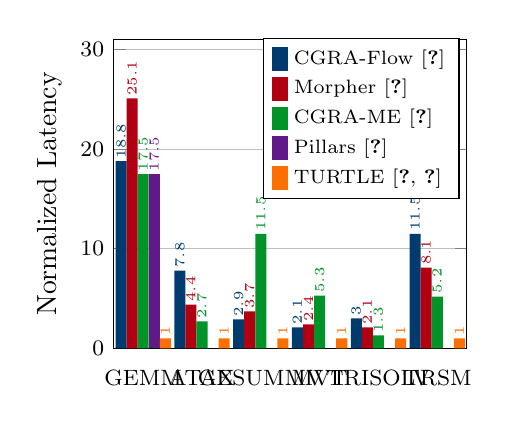
\begin{tikzpicture}
        \definecolor{darkPurple}{RGB}{96, 25, 134}   
        \definecolor{darkBlue}{RGB}{0, 59, 111}      
        \definecolor{darkBrown}{RGB}{102, 51, 0}     
        \definecolor{darkGray}{RGB}{71, 79, 82}   
        \definecolor{darkRed}{RGB}{177, 0, 18}
        \definecolor{darkGreen}{RGB}{0, 147, 39}
        \definecolor{darkCyan}{RGB}{0, 147, 146}
        \definecolor{darkOrange}{RGB}{255, 111, 0}
        \begin{axis}[
            width  = 0.5*\textwidth,
            height = 5.5cm,
            major x tick style = transparent,
            ybar=0pt, %2*\pgflinewidth,
            bar width=4pt,
            ymajorgrids = true,
            ylabel = {Normalized Latency},
            tick label style = {font=\footnotesize},
            symbolic x coords={GEMM, ATAX, GESUMMV, MVT, TRISOLV, TRSM},
            xtick = data,
            scaled y ticks = false,
            ymax=31,
            ymin=0,
            legend image code/.code={
            \draw [#1] (0cm,-0.15cm) rectangle (0.2cm,0.15cm); },
            legend style={font=\scriptsize,yshift=0.1cm},
            legend cell align={left},
            nodes near coords,
            nodes near coords style = {font=\tiny,rotate=90,anchor=west,inner sep=0.03cm},
        ]
            \addplot[style={fill=darkBlue, darkBlue,draw opacity=0}]
                coordinates {(GEMM,18.8) (ATAX,7.8) (GESUMMV,2.9) (MVT,2.1) (TRISOLV,3.0) (TRSM,11.5)};

            \addplot[style={fill=darkRed,darkRed,mark=none, draw opacity=0}]
                coordinates {(GEMM,25.1) (ATAX,4.4) (GESUMMV,3.7) (MVT,2.4) (TRISOLV,2.1) (TRSM,8.1)};

            \addplot[style={darkGreen, fill=darkGreen,mark=none, draw opacity=0}]
                coordinates {(GEMM,17.5) (ATAX,2.7) (GESUMMV,11.5) (MVT,5.3) (TRISOLV,1.3) (TRSM,5.2)};

            \addplot[style={darkPurple, fill=darkPurple,mark=none, draw opacity=0}]
                coordinates {(GEMM,17.5) };

            \addplot[style={darkOrange, fill=darkOrange,mark=none, draw opacity=0}]
                coordinates {(GEMM,1.0) (ATAX,1.0) (GESUMMV,1.0) (MVT,1.0) (TRISOLV,1.0) (TRSM,1.0)};

            \legend{%
                CGRA-Flow~\cite{4_OpenCGRA}, Morpher~\cite{6_MorpherWOSET}, CGRA-ME~\cite{RaghebWWBRYA24}, Pillars~\allowbreak\cite{guo-pillars-woset2020}, TURTLE~\cite{WitteraufWHT21, TanaseHannig2018ATECS}
            }
        \end{axis}
    \end{tikzpicture}
    \caption{%
        Speedup of TURTLE-compiled loop nests compared to other CGRA frameworks for an input matrix size of $20 \times 20$ for GEMM and $32 \times 32$ for all other benchmarks and assuming an array size of $4\times 4$ PEs.
    }
    \label{fig:barChart}
\end{figure}
